\chapter{Results} \label{chapter:results}

% overview of runs
% explanation of the dashboard view
% dashboard results
% resultant mesh results

For each experimental run, a dashboard view was created that can be shown for
each iteration of the simulation. The dashboard view combines several different
views of information useful for understanding the inner workings of the MABDI
algorithm. As an example, Figure \ref{fig:run1} shows the dashboard view for the
first experimental run. For these experiments, all dashboard views follow the
same pattern as described below:

\begin{itemize}
  \item (a) - Shows the global mesh $M$ from a third-person point of view and in
  the context of the simulated environment. The multi-colored mesh is $M$. The
  mesh is multi-colored in order to show the passage of time. For example, in
  Run1, The mesh is colored yellow, light green, and dark green for iterations
  1, 2, and 3 respectively. Additional items in the view show elements of the
  simulated environment: the wire frame corresponds to the viewing frustum of
  the sensor, the light blue helical line is the path of the sensor, and the
  translucent gray mesh is the simulated environment.
  \item (b) - Same as (a) except it shows the novel surface $S$ instead of
  the global mesh $M$.
  \item (c) - Plot showing the number of elements in the global mesh $M$
  after this iteration.
  \item (d \& e) - Actual $D$ and expected $E$ depth image
  respectively.
  \item (f) - The classified depth image. Points that will be used to generate
  the novel surface $S$ are shown in black. Points to be thrown away are shown
  in white.
\end{itemize}

The dashboard views are an excellent way to visualize important aspects of
MABDI. In the next section, Section \ref{section:results1}, we will utilize key
dashboard views to look at the behavior and performance of MABDI at one particular iteration of each experimental run. In section \ref{section:results2} we will analyze the
quality and progression of the resultant global mesh from each experiment.

\section{MABDI Performance During Experiments}
\label{section:results1}

\subsection{Experiment 1}

Figure \ref{fig:run1} shows the dashboard view of the first experiment during
the third iteration. Note that \ref{fig:run1}(a) shows $M$ after the third
iteration. As stated before, $M$ is multi-colored in order to show the passage
of time. The mesh is colored yellow, light green, and dark green for iterations
1, 2, and 3 respectively. \emph{During iteration 3, $M$ is composed of only the
yellow and light green parts.}

\begin{figure}[h]%[thpb]
\centering
  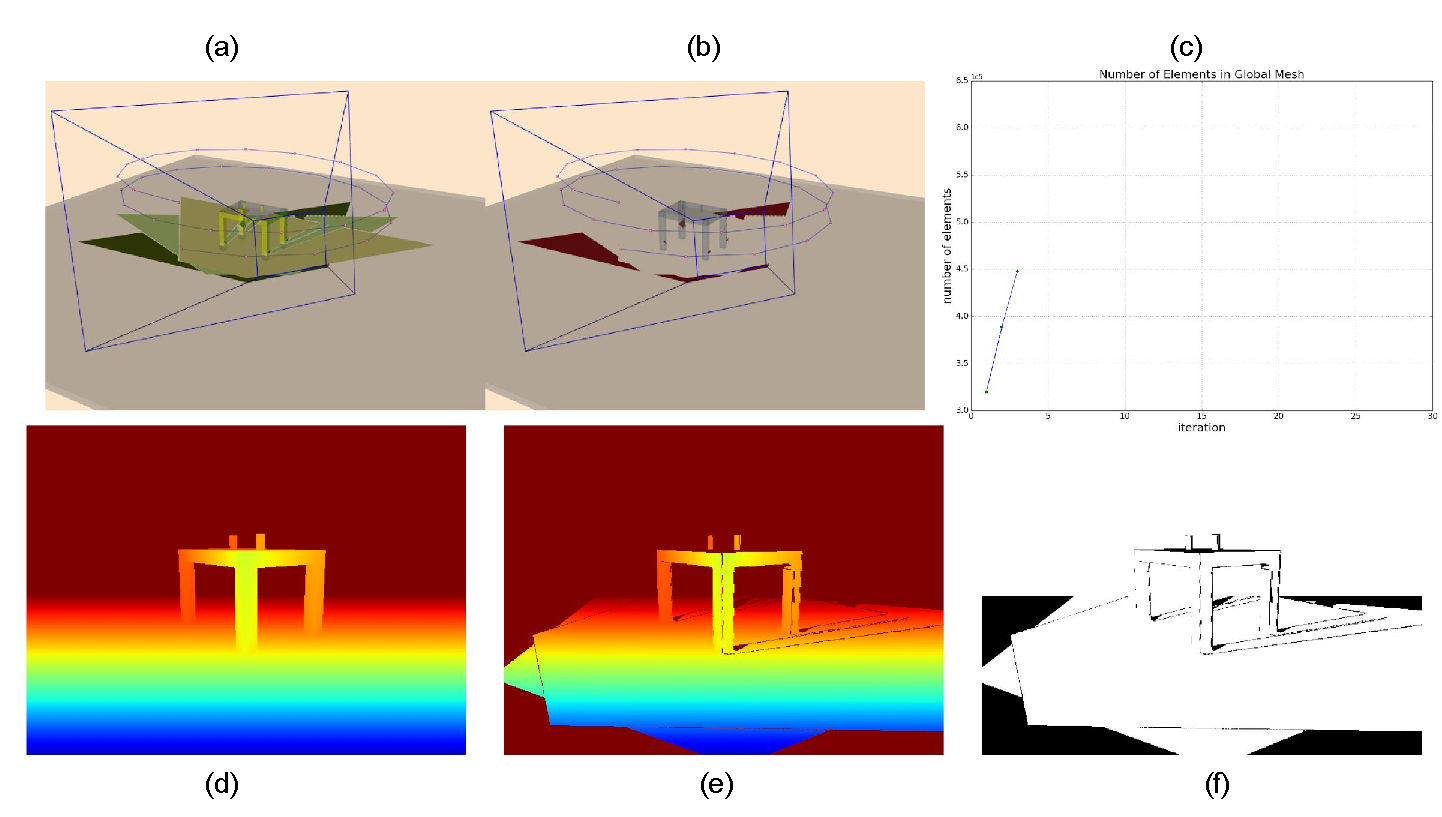
\includegraphics[width=\textwidth]{figures/diagram_run1.pdf}
  \caption{Dashboard view of the first experimental run.}
  \label{fig:run1}
\end{figure}

Examining Figure \ref{fig:run1} demonstrates how the novel surface
$S$ is appended to the global mesh $M$ after each iteration of MABDI. Let's use
the figure to follow the process. It will be useful to refer to Figure
\ref{fig:system} for this section.

\begin{sloppypar} % to get rid of weird black box thing
\begin{enumerate}
  \item Input - \ref{fig:run1}(d) shows the depth image $D$ generated from the
  simulated sensor. \ref{fig:run1}(a) shows us two important aspects to consider
  about $D$. First, the pose $P$ of the sensor is shown by looking at the
  sensor's view frustum, indicated by the blue wireframe. Second, the only
  environmental information used to generate the depth image is shown in light
  gray.
  \item Generate Expected Depth Image ($E$) - \ref{fig:run1}(e) shows the
  expected depth image $E$. \ref{fig:run1}(a) also shows us two important
  aspects to consider about $E$. First, the same pose $P$ is used to create both
  $D$ and $E$ (as indicated by the blue wire frame). Second, the only
  environmental information used to create $E$ is the yellow and light green
  parts of $M$ because that is the only information $M$ contains \emph{during}
  iteration 3.
  \item Classify Depth Image ($D$) - \ref{fig:run1}(f) visualizes the
  classification process. More specifically, it shows the points as expressed in
  Equation \ref{eqn:throwaway} in white ($D_{throwaway}$). \ref{fig:run1}(f) is
  important for understanding how MABDI works because it clearly shows which
  points will be thrown away (white) and which points will be kept for
  generating the novel surface $S$ (black).
  \item Surface Reconstruction - \ref{fig:run1}(b) shows the novel surface $S$
  in the context of the simulated environment. $S$ is constructed using all the
  points colored black in \ref{fig:run1}(f).
  \item Add Novel Surface ($S$) to Global Mesh($M$) - \ref{fig:run1}(a) shows
  the novel surface $S$ appended to the global mesh $M$ in dark green.
\end{enumerate}
\end{sloppypar}

\subsection{Experiment 2}

The second experiment gives us a clear example of how the classification process
is able to identify points from the depth image $D$ that correspond to parts of
the environment that have not been seen before. In this example the global mesh
$M$ has a partial representation of the objects in the environment and when the
sensor is moved to the next pose $P$, the new perspective reveals a portion of
the object that has not been seen before. This \emph{novel portion} of the
environment, which we will be referring to, is shown by the red ellipse in Figure
\ref{fig:run2_novel_portion}.

\begin{figure}[h]%[thpb]
\centering
  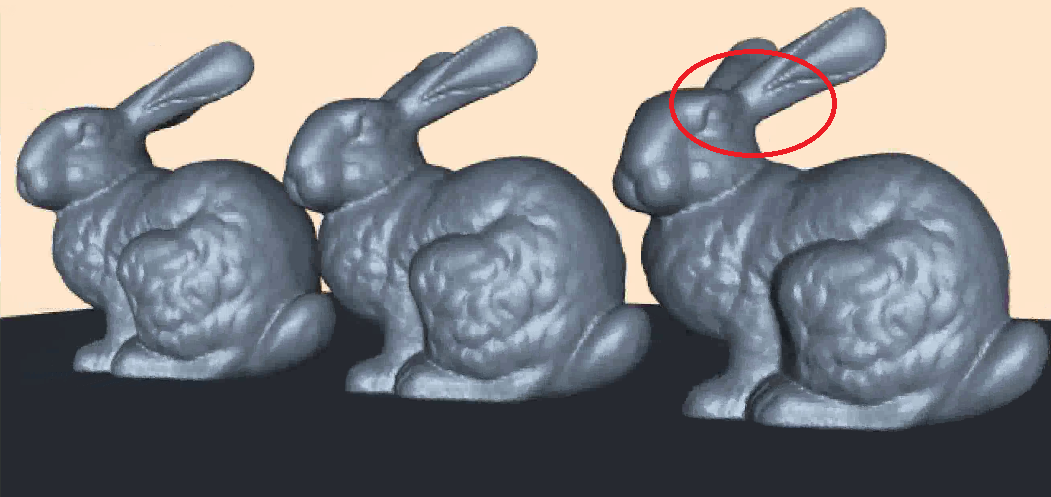
\includegraphics[width=0.8\textwidth]{figures/run2_novel_portion.png}
  \caption{\emph{Novel portion} of the environment that we will be referring to
  in this section.}
  \label{fig:run2_novel_portion}
\end{figure}

Figure \ref{fig:run2} shows the dashboard view of the second experiment during
the second iteration. Using the dashboard view, we can follow how MABDI handles
the novel portion of the object step-by-step:
\begin{enumerate}
  \item \ref{fig:run2}(a) shows the global mesh $M$. The yellow portion of the
  mesh constitutes the entirety of $M$ after the first iteration. We can see the
  novel portion of the environment was not represented in $M$ after the first
  iteration due to occlusion.
  \item \ref{fig:run2}(d) shows the depth image $D$ from the new sensor pose
  $P$. We can see the novel portion can be seen by the sensor on this iteration.
  \item \ref{fig:run2}(e) shows the expected depth image $E$. During the second
  iteration $M$ consists of only the yellow portion shown in \ref{fig:run2}(a)
  consequently, $E$ does not show any points in the area corresponding to the
  novel portion of the environment.
  \item \ref{fig:run2}(f) shows the classification process successfully
  identifying points in $D$ that correspond to the novel portion as indeed
  novel. In the figure the points are highlighted by a red circle.
  \item \ref{fig:run2}(b) shows the novel surface $S$ now represents the novel
  portion of the environment.
  \item Finally, the orange mesh in \ref{fig:run2}(a) shows the novel portion of
  the environment is now represented by the global mesh $M$.
\end{enumerate}

\begin{figure}[h]%[thpb]
\centering
  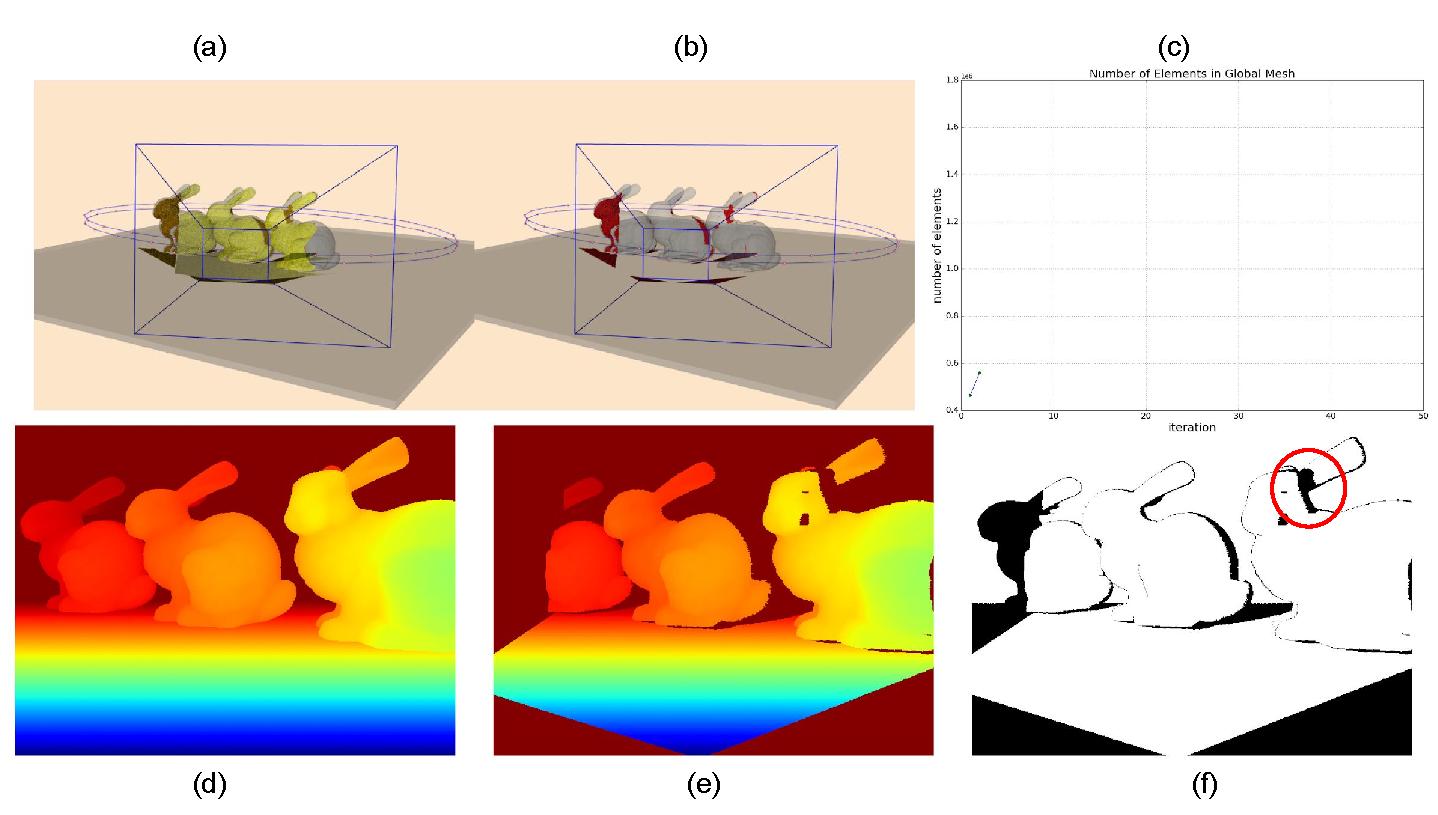
\includegraphics[width=\textwidth]{figures/diagram_run2.pdf}
  \caption{Dashboard view of the second experimental run.}
  \label{fig:run2}
\end{figure}

\subsection{Experiment 3}

Experiment three shows how MABDI reacts to object addition. Figure
\ref{fig:run3} shows the dashboard view of the third experiment during the
twenty-sixth iteration. At this iteration the middle bunny is suddenly added to
the simulated environment. We can use the dashboard view to see the behavior of
MABDI to this new object:
\begin{enumerate}
  \item In \ref{fig:run3}(d) we see the depth image $D$ shows the new bunny.
  \item In \ref{fig:run3}(e) the expected depth image $E$ does not show the new
  bunny because $M$ has no representation of the new bunny.
  \item \ref{fig:run3}(f) shows the classification process successfully
  identified the points corresponding to the new bunny as novel.
  \item The novel points are used to generate the novel surface $S$ and then $S$
  is appended to $M$, shown in \ref{fig:run3}(a \& b).
  \item The addition of the new object resulted in a $S$ with a large number of
  elements for this particular iteration. \ref{fig:run3}(f) plots the resulting
  jump in the number of elements contained with $M$.
\end{enumerate}

\begin{figure}[h]%[thpb]
\centering
  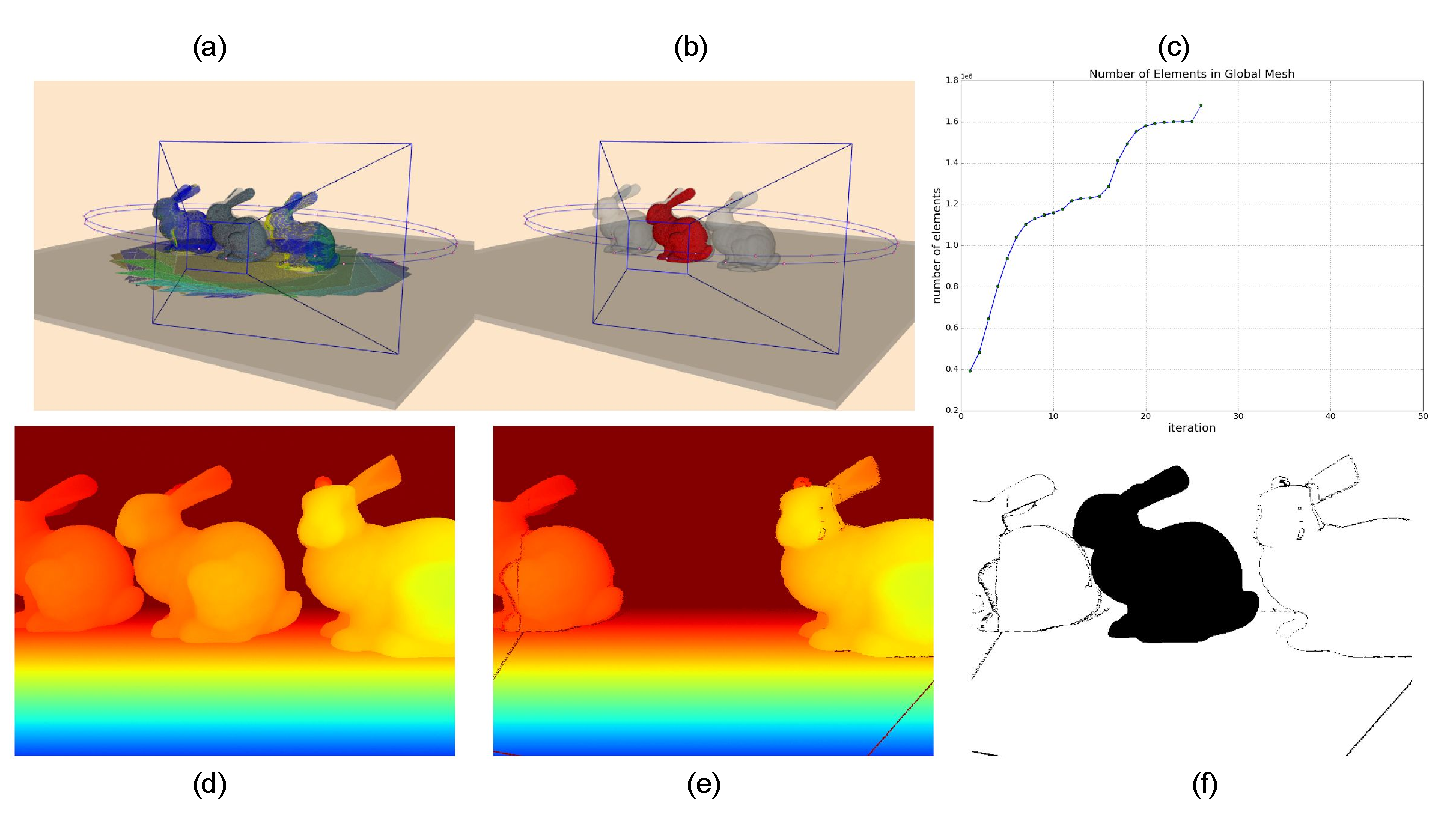
\includegraphics[width=\textwidth]{figures/diagram_run3.pdf}
  \caption{Dashboard view of the third experimental run.}
  \label{fig:run3}
\end{figure}

\section{Global Mesh Results}
\label{section:results2}

\subsection{Mesh Quality}

% quality of the mesh
Figure \ref{fig:gm_3_full} shows the resultant global mesh from experiment 3. In
this section we will use this figure to make observations about the quality of
the global mesh for all three experiments.

There are gaps in the mesh that occur typically along the boundaries
of where the novel surface $S$ is appended to the global mesh $M$. This behavior
is common for Surface Reconstruction methods as those discussed in Section
\ref{section:surface_reconstruction}. Algorithms exist for merging these gaps as
a post processing step such as Turk's Zippered Polygon Meshes \cite{Turk1994}.
The aforementioned methods are typical for single object reconstruction.
Traditional mesh-based environmental mapping algorithms simply append
overlapping layers of mesh resulting in no gaps but a heavily redundant
representation with a high memory cost.

The mesh is noisy. This noisiness is due to the simplicity of our
implementation's surface reconstruction method as discussed in Section
\ref{subsection:surface_reconstruction}. Our method simply connects neighboring
points in the point cloud without additional steps such as Laplacian smoothing
\cite{Nealen2006}. Our reconstruction method was sufficient for
demonstrating the usefulness of the MABDI algorithm, but results in a mesh with
the same magnitude of noise as the sensor's simulated noise.

\begin{figure}[h]%[thpb]
\centering
  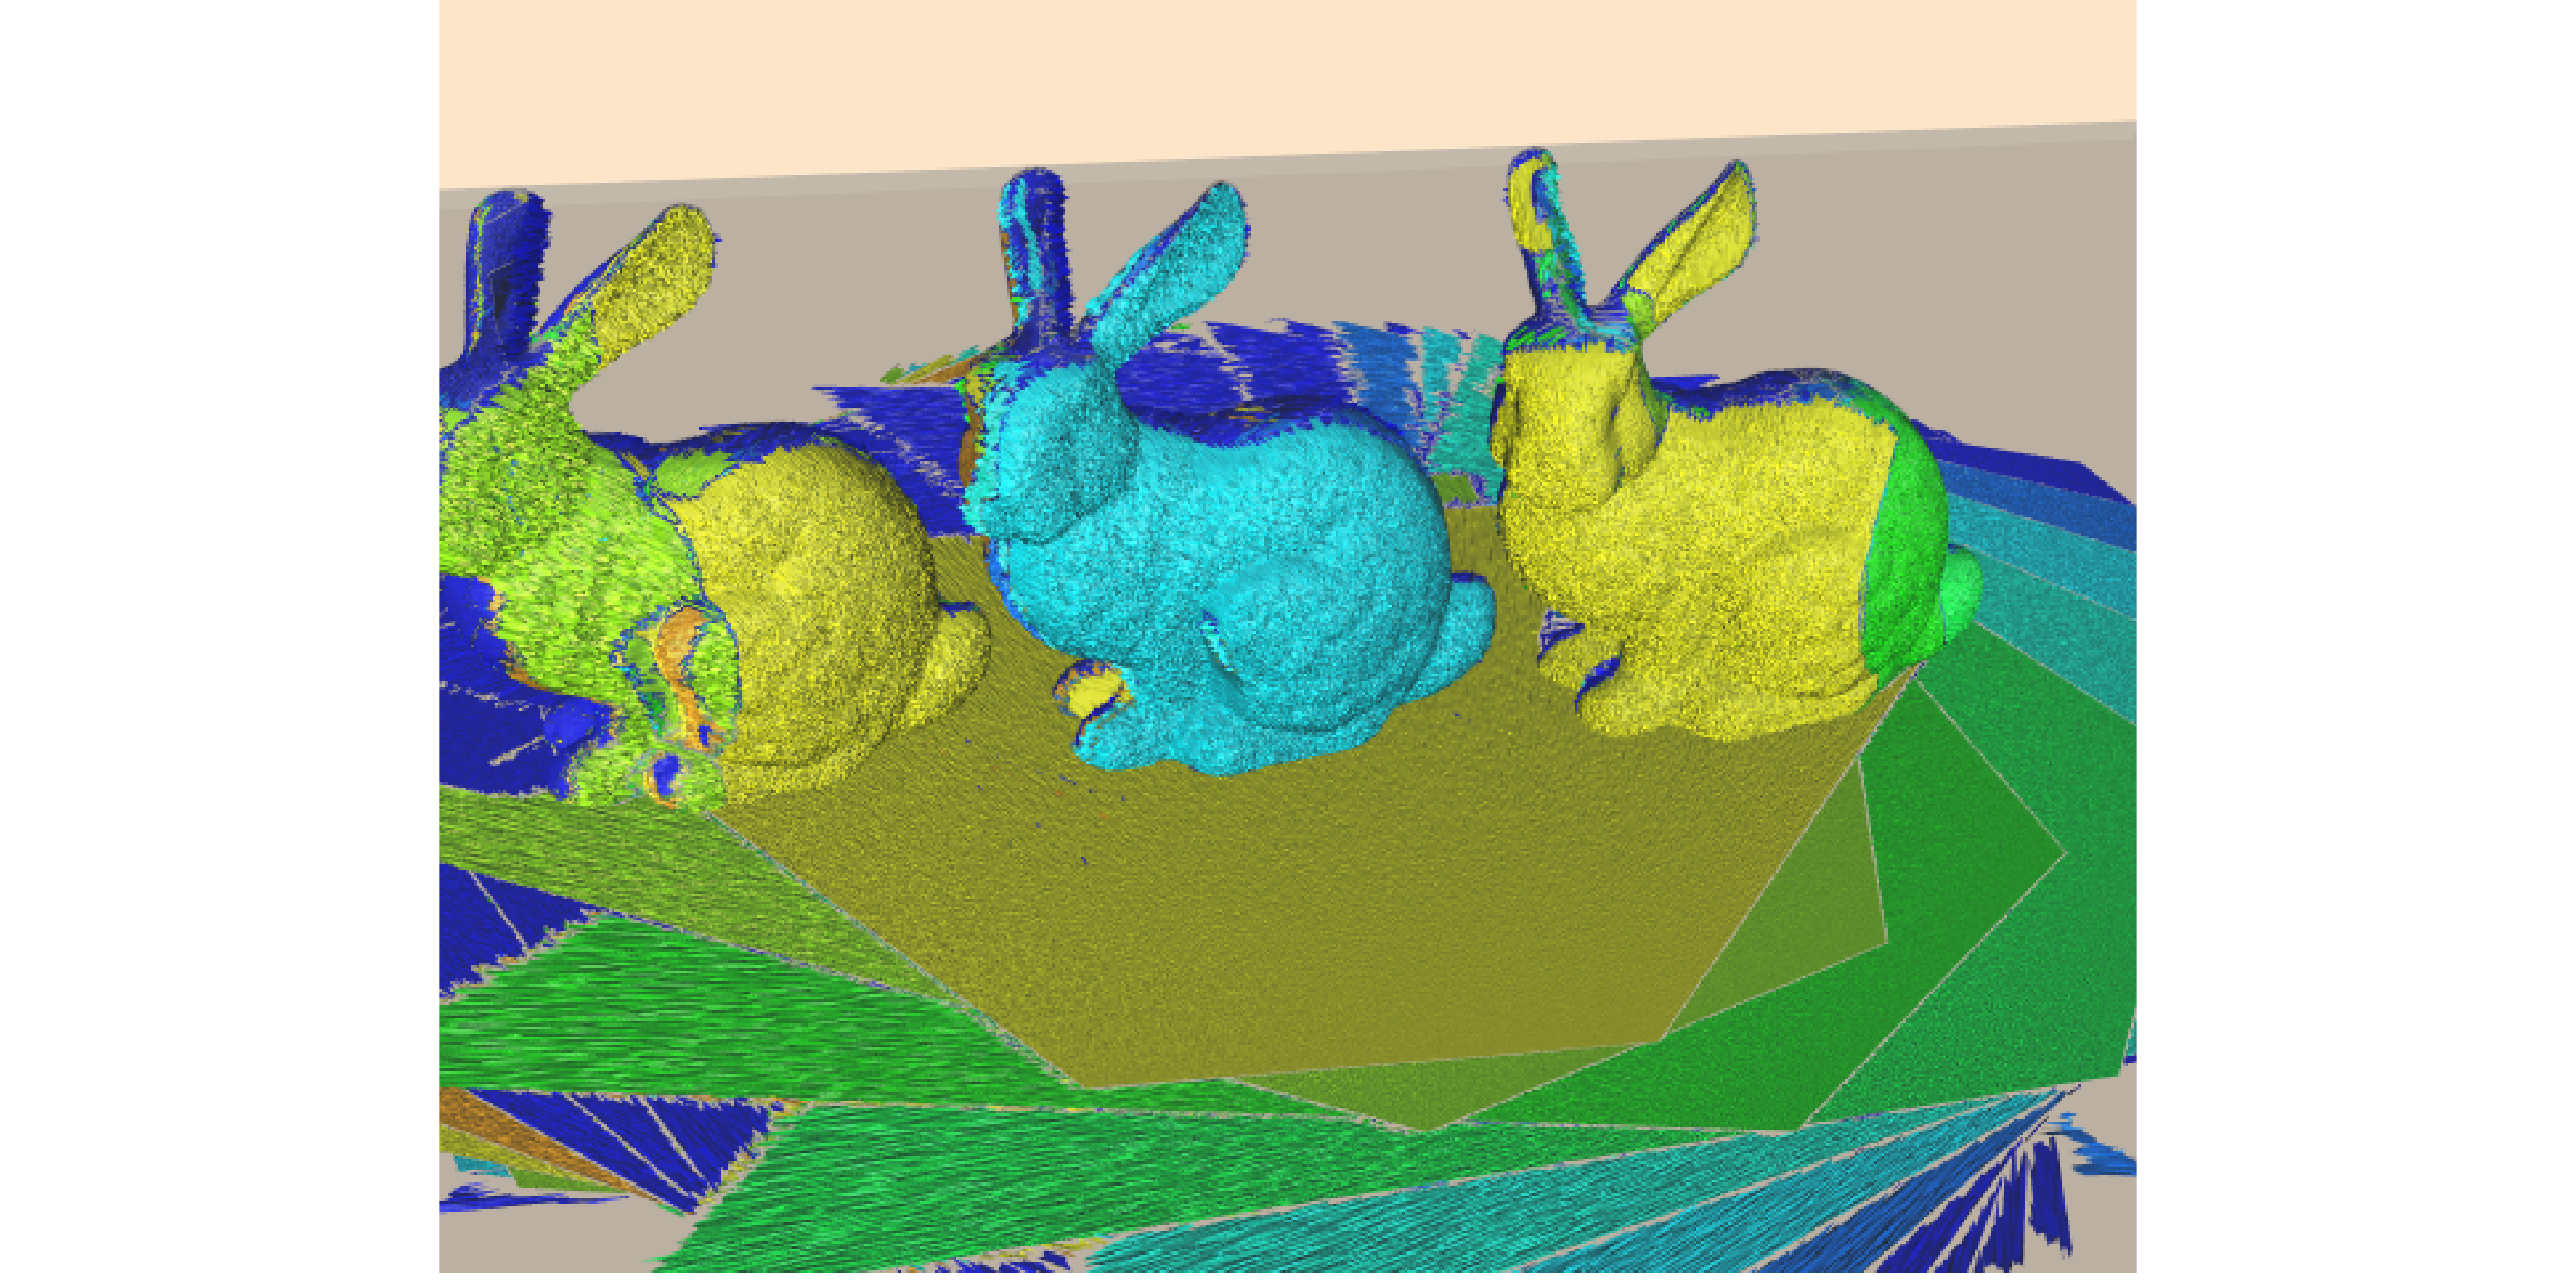
\includegraphics[width=\textwidth]{figures/run3_global_mesh.png}
  \caption{Global mesh at the end of experiment 3.}
  \label{fig:gm_3_full}
\end{figure}

\subsection{Mesh Progression}

% shape of the graphs
To appreciate the true benefit of the MABDI algorithm it is helpful to look at
how the number of elements in the global mesh $M$ progress over time. In this
section we will analyze plots showing how the number of elements in $M$ change
during the experiments. Note, the dashboard views also showed this plot. For
example, the plot of Figure \ref{fig:gm_1} is the same as Figure
\ref{fig:run1}(c), but Figure \ref{fig:gm_1} shows the plot at the completion of
the experiment.

Figure \ref{fig:gm_1} shows the resultant mesh and mesh progression for the
first experiment. The plot highlights the major difference between MABDI
and traditional mesh-based environmental mapping methods. Traditional methods
would have a plot similar to that indicated by the red arrow on the graph
because these methods have no ability to identify or remove redundant mesh
elements. Due to MABDI's algorithmic design, MABDI has the intrinsic ability to
identify points in the depth image corresponding to parts of the environment
that are already known by the global mesh $M$. MABDI then simply does not use
those points for surface reconstruction and consequently does not create
redundant mesh elements. For this reason, the number of elements in $M$ levels
off as the environment becomes more known.

\begin{figure}[h]%[thpb]
\centering
  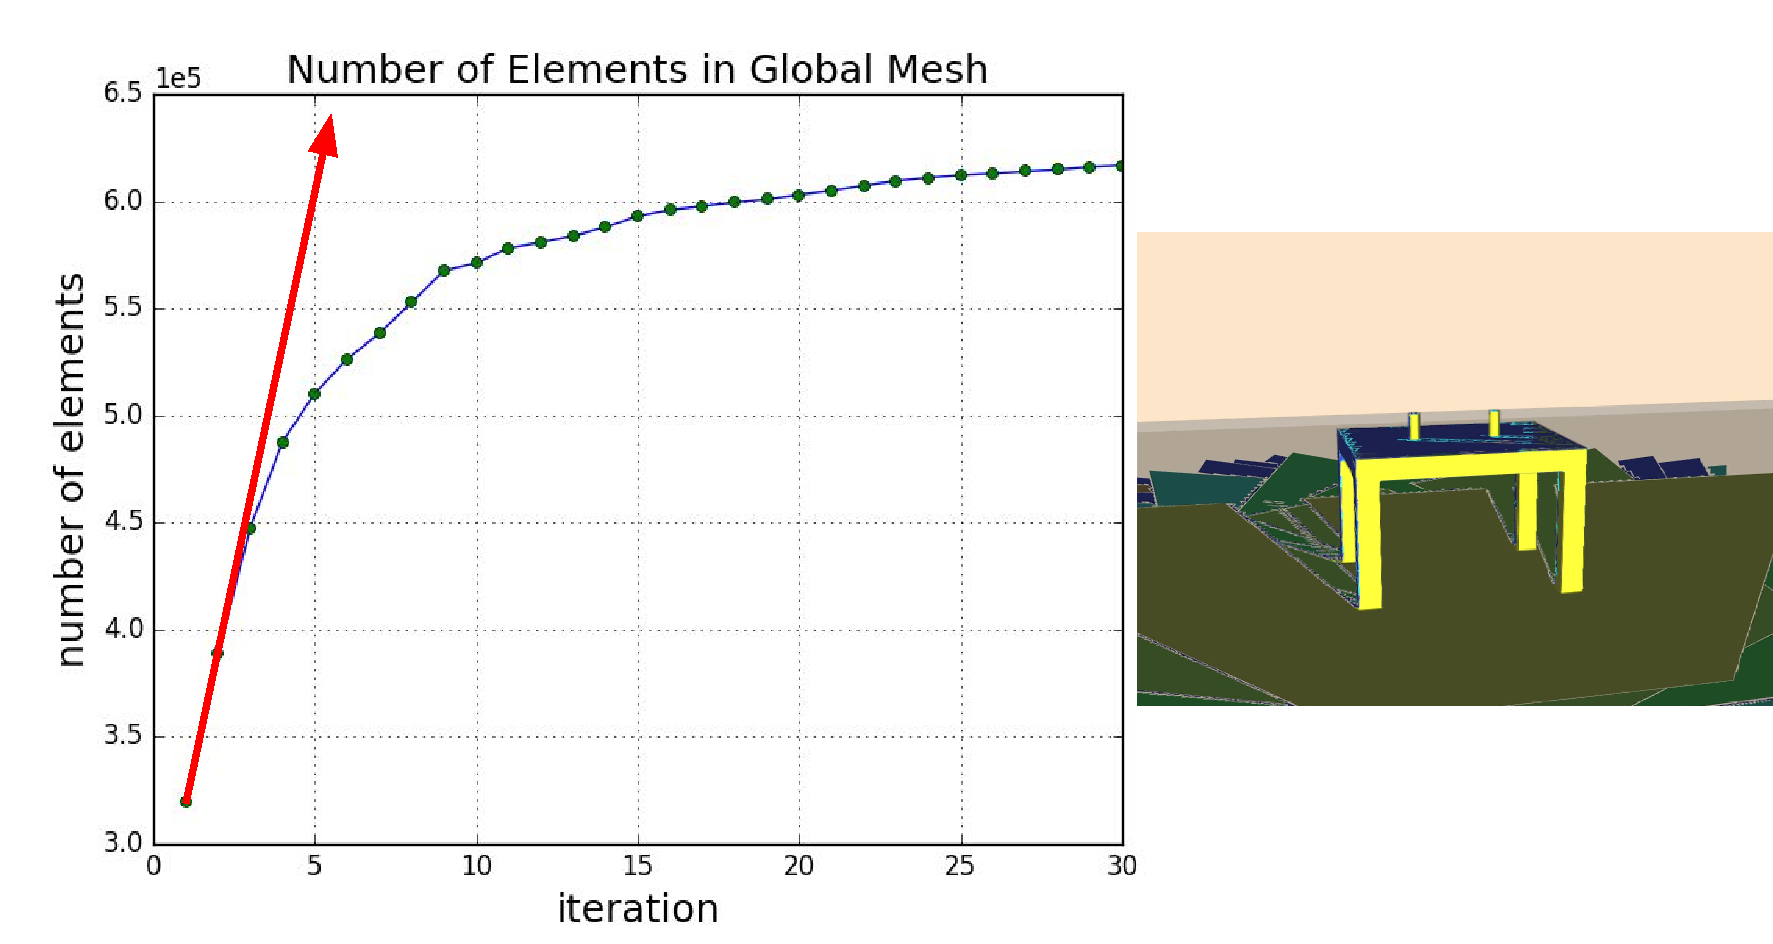
\includegraphics[width=\textwidth]{figures/diagram_run1_gm.pdf}
  \caption{Experiment 1 global mesh results.}
  \label{fig:gm_1}
\end{figure}

Figure \ref{fig:gm_2} shows us the resultant mesh after the second experiment.
Here we can see that MABDI is reactive to the environment. In the preceding
experiment, the environment was symmetrical. In this experiment, the environment
is not symmetrical and we can see the effects by looking at the progression of
the global mesh $M$. First let us note that the sensor circles the objects twice
during the experiment and in total travels $720^{\circ}$ during the 50
iterations. We notice when the sensor gets to $90^{\circ}$ (around iteration
7) the number of elements begins to level off and then increases again as the
sensor travel to $270^{\circ}$ (around iteration 19). This behavior occurs
because the information rich perspectives of the environment occur at
$0^{\circ}$ and $180^{\circ}$. There is less for the sensor to look at when
viewing the environment from the sides. In this way, MABDI is reactive as the
sensor moves to parts of the environment that are rich in information.
Consequently, the mesh grows rapidly based on the needs of the environment.

\begin{figure}[h]%[thpb]
\centering
  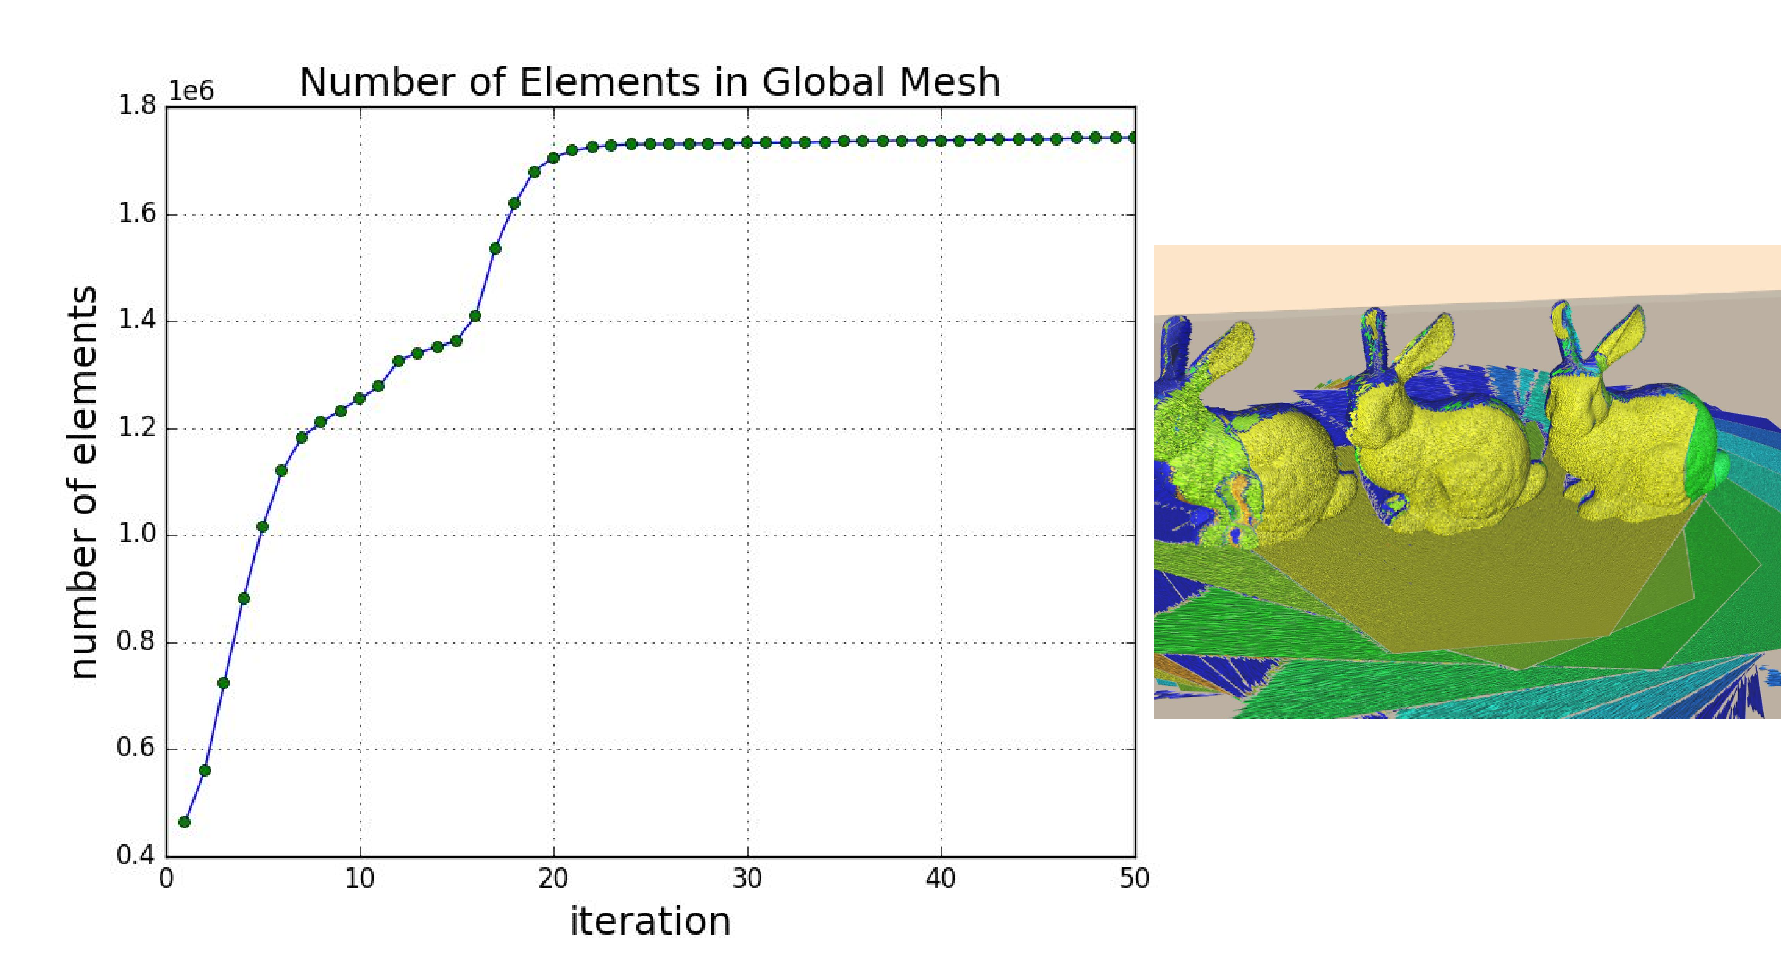
\includegraphics[width=\textwidth]{figures/diagram_run2_gm.pdf}
  \caption{Experiment 2 global mesh results.}
  \label{fig:gm_2}
\end{figure}

Figure \ref{fig:gm_3} shows us the resultant mesh after the third experiment. In
this experiment the middle bunny was added during the twenty-sixth iteration.
This object addition had two effects on the global mesh. First, it created a
sudden jump in the plot as highlighted by the red circle. Second, the middle
bunny is colored blue in the resultant mesh, signifying that it was added to $M$
during a different iteration than the bunnies on the left and the right. Both of
these effects indicate that MABDI was able to successfully identify the new
bunny as novel and incorporate the bunny in to the global mesh within one
iteration.

\begin{figure}[h]%[thpb]
\centering
  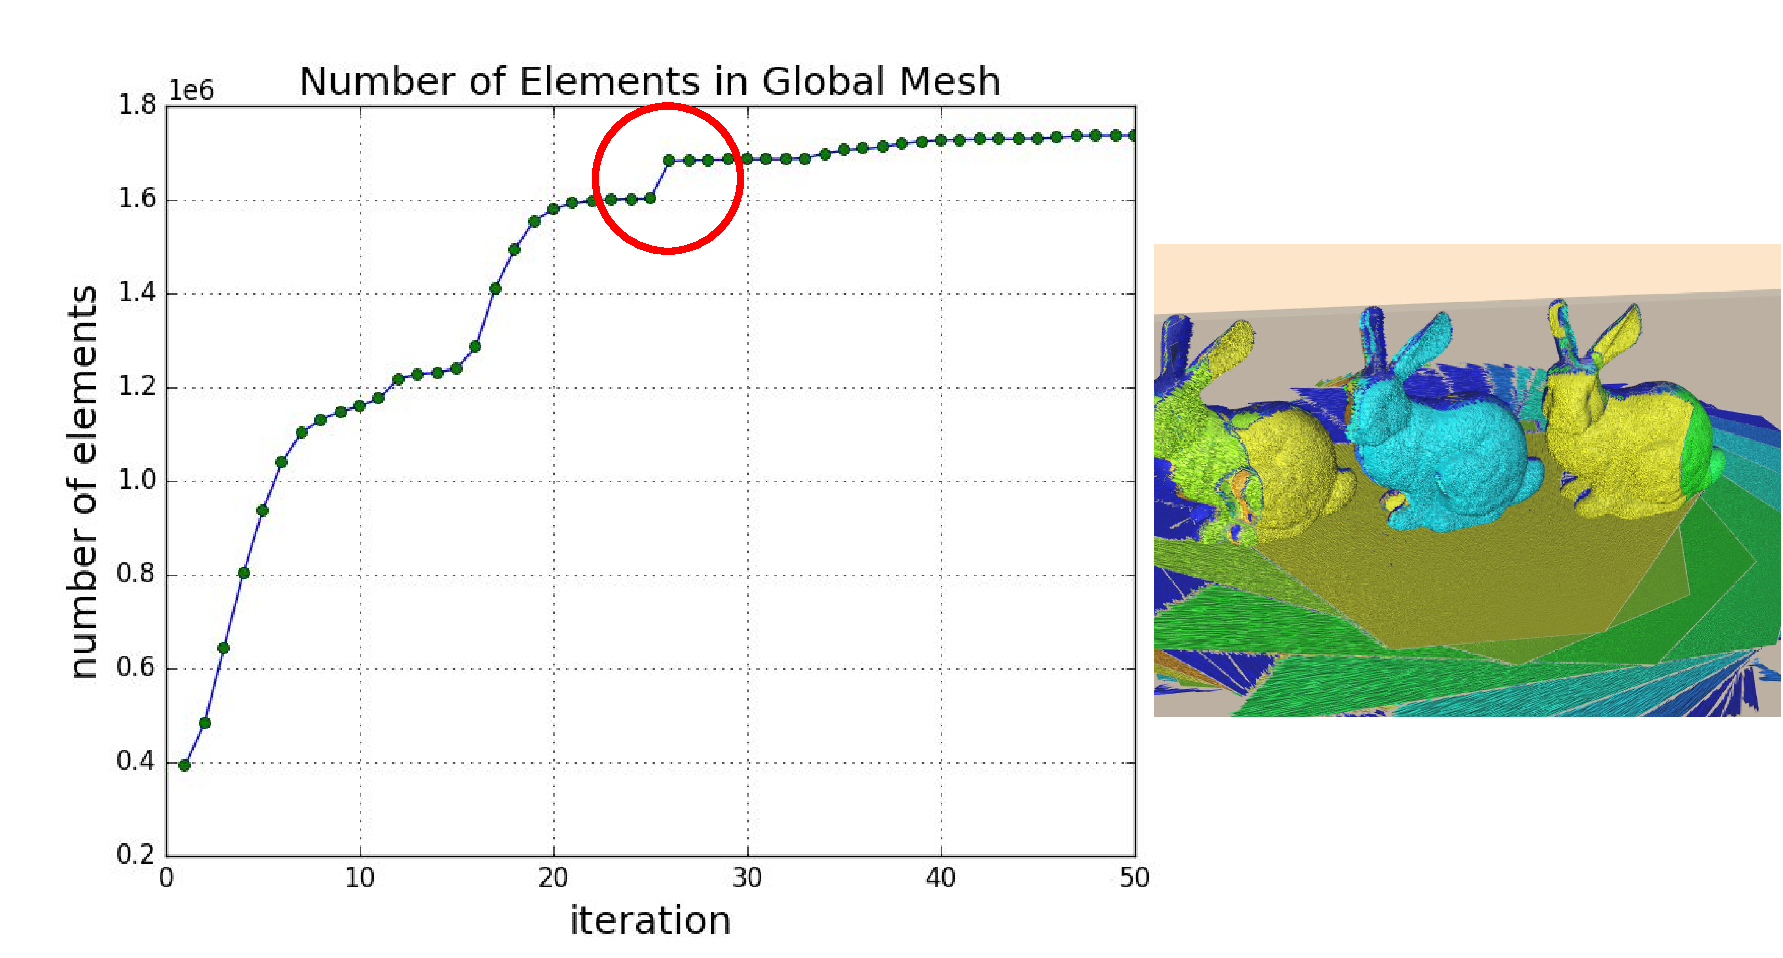
\includegraphics[width=\textwidth]{figures/diagram_run3_gm.pdf}
  \caption{Experiment 3 global mesh results.}
  \label{fig:gm_3}
\end{figure}

% Figure \ref{fig:gm} shows the resultant global mesh $M$ for each of the experiments
% along with a plot of the number of elements in the mesh over iterations. These
% plots show the main contribution of MABDI because they level-off as the
% environment becomes more known as opposed to traditional reconstruction methods
% where the number of elements increases linearly over time.
